	\documentclass[ucs, notheorems, handout]{beamer}
	
	\usefonttheme[onlymath]{serif}
	\setbeamertemplate{navigation symbols}{}
	
	%\mode<handout> {
	%    \usepackage{pgfpages}
	%    \setbeameroption{show notes}
	%    \pgfpagesuselayout{2 on 1}[a4paper, border shrink=3mm]
	%}
	
	\usepackage[utf8x]{inputenc}
	\usepackage[T2A]{fontenc}
	\usepackage[russian]{babel}
	\usepackage{tikz}
	\usepackage{ragged2e}
	\usepackage{amsthm}
	\usepackage{wrapfig}
	\usepackage{bm} %bold math
	\usepackage{url}
	\usepackage{dirtytalk} %for quotes
	\usepackage{graphicx}
	\usepackage{marginnote}
	\usepackage{bm}
	\usepackage[makeroom]{cancel}
	\usepackage{algorithm2e}
	\newcommand{\sign}{\text{sign}}
	\DeclareMathOperator*{\argmax}{arg\,max}
	\DeclareMathOperator*{\argmin}{arg\,min}
	\DeclareMathOperator{\rank}{rank}
	\DeclareMathOperator{\diam}{diam}
	\DeclareMathOperator{\ob}{Ob}
	\DeclareMathOperator{\Hom}{Hom}
	\DeclareMathOperator{\var}{Var}
	\DeclareMathOperator{\bias}{Bias}
	\newcommand{\betah}{\hat{\bm \beta}}
	\newcommand{\betaa}{\bm{\beta}}
	\newcommand{\epss}{\bm{\varepsilon}}
	\newcommand{\E}{\mathrm{E}}
	\newcommand{\D}{\mathrm{D}}
	\newcommand{\XT}{{\bm{X}}^{\mathrm{T}}}
	\newcommand{\X}{\bm{X}}
	\renewcommand{\thealgocf}{}
	\definecolor{asparagus}{rgb}{0.53, 0.66, 0.42}
	
	\newtheorem{theorem}{Теорема}
	\newtheorem{definition}{Определение}
	\addto\captionsrussian{\renewcommand{\figurename}{Figure}}
	\addto\captionsrussian{\renewcommand{\tablename}{Table}}
	
	\title[Регрессия, регуляризация, работа с признаками]{%
	     Регрессия, регуляризация, работа с признаками}
	
	\author[Михайлов Дмитрий, Cмирнов Иван]{Михайлов Дмитрий, Cмирнов Иван}
	
	\institute[Санкт-Петербургский Государственный Университет]{%
	    \small
	    Санкт-Петербургский государственный университет\\
	    Кафедра статистического моделирования\\
	    \vspace{1.25cm}
	}
	
	\date[]{Санкт-Петербург, 2023}
	
	%\subject{Talks}
	
	\begin{document}
	
	\begin{frame}[plain]
	    \titlepage
	\end{frame}
	
	
	\begin{frame}
	    \frametitle{Идея}
	
	
	Имеется набор данных (обучающая выборка)
	$$
	\X \in \mathbb{R}^{n\times p}, \quad \bm y \in \mathbb R^n
	$$ 
	\vspace{0.5cm}   
	$\mathbf x_i \in \mathbb R^p$ --- вектор-строки $\X$, $X_i \in \mathbb R^n$ --- вектор-столбцы $\X$.
	
	\textbf{Задача:} уметь предсказывать $y$ (ответ) по новым $\mathbf x_i$ (объектам), установив некоторую зависимость на обучающей выборке.
	\vspace{0.5cm}  
	
	\end{frame}
	
	
	
	
	
	
	\begin{frame}
	    \frametitle{Постановка задачи}
	    \vspace*{-5mm}
	\begin{center}
		\textbf{"До эксперемента":}
	\end{center}
	
	$\bm \xi \in \mathbb R^p$ --- случайный вектор, $\eta, \varepsilon \in \mathbb R$ --- случайные величины.
	
	Предполагаем, что $\eta$ и $\bm \xi$ функционально зависимы:
	\begin{block}{}
	\centering
	$\eta = \varphi(\bm \xi) + \varepsilon$
	\end{block}
	Обычно $\E \varepsilon = 0, \, \D \varepsilon = \sigma^2,\, \bm\xi \perp \varepsilon. $
	\begin{center}
	\textbf{"После эксперемента":}
	\end{center}
	$\mathbf x_1, \ldots, \mathbf x_n \sim \mathcal L(\bm \xi)$; $y_1, \ldots, y_n \sim \mathcal L(\eta)$ --- выборки, которые наблюдаем.
	Модель для всех $i \in 1:n$ 
	\begin{block}{}
	\centering
	$y_i = \varphi(\mathbf x_i) + \varepsilon_i$
	\end{block}
	
	\textbf{{\color{blue}{Задача:}}} найти функцию $\varphi$.
	
	\end{frame}
	
	\begin{frame}
	    \frametitle{Этапы обучения модели}
	\begin{block}{Модель}
	$$
	y_i = \varphi(\mathbf x_i) + \varepsilon_i
	$$
	\end{block}
	\textbf{\color{blue}{Задача:}} найти функцию $\varphi$.
	\vspace{3mm}
	\begin{enumerate}
		\item Выбор модели регрессии (класс рассматриваемых $\varphi(\cdot)$)
		
		{\color{gray} Линейная модель: $\varphi(\mathbf x_i, \betaa) = \sum_{j = 1}^p \beta_i \mathbf x_i[j],\quad i \in 1:n $}
		
		\item Выбор функции потерь (loss function)
		
		{\color{gray} Квадратичная функция потерь: $\sum_{i = 1}^n(y_i - \varphi(\mathbf x_i, \betaa))^2$}
		\item Выбор метода обучения (training)
	
	{\color{gray} МНК: $\betah = \argmin_{\betaa}{\sum_{i = 1}^n(y_i - \varphi(\mathbf x_i, \betaa))^2}$}
		\item Выбор метода проверки (test)
	
	{\color{gray} MSE: $\tfrac{1}{n_{\text{test}}}\sum_{i = 1}^{n_{\text{test}}}(y^{\text{test}}_i - \varphi(\mathbf x_i^{\text{test}}, \betah))^2$}
	\end{enumerate}            
	\end{frame}
	
	
	\begin{frame}
	    \frametitle{Оптимизация. Матричный вид в общем случае}
	\begin{itemize}
		\item $\X \in \mathbb R^{n \times p}$ --- матрица данных
		\item $\bm y \in \mathbb R^n$ --- вектор ответов
		\item $\betaa \in \mathbb R^d$ --- вектор параметров 
		\item $\bm \varphi(\X, \betaa) := (\varphi(\mathbf x_1, \betaa),\ldots, \varphi(\mathbf x_n, \betaa) )^\mathrm T$ --- функция от выборки и параметров	\item $\mathcal L(\bm \varphi(\X, \betaa), \bm y)$ --- \textit{некоторая} функция потерь
	\end{itemize}
	Решение задачи регрессии --- вектор коэффициентов $\betah$. 
	\begin{block}{}
	$$\betah = \argmin_{\betaa}{\mathcal L(\bm \varphi(\X, \betaa), \bm y)}$$
	\end{block}
	\end{frame}
	
	\begin{frame}
	    \frametitle{Выбор функции потерь}
	\textit{Какие варианты есть?}
	\begin{itemize}
		\item $\|\bm \varphi(\bm X, \betaa) - \bm y\|^2_2$ --- квадратичная ошибка ($l_2$-норма)
		\item $\|\bm \varphi(\bm X, \betaa) - \bm y\|_1$ --- модуль ошибки ($l_1$-норма)
	\end{itemize}
	    \vspace{3mm}
	\textit{Как выбирать?}
	\begin{itemize}
		\item Предположения о распределении остатков $\bm \varepsilon$
		\item Простота функции $\mathcal L$ для оптимизации
		\item Точность данных/наличие выбросов
	\end{itemize}
	\end{frame}
	
	\begin{frame}
	    \frametitle{Линейная регрессия: постановка}
	    \textbf{Модель:	} $\bm y = \X \betaa + \epss$
	\begin{itemize}
		\item $\bm y \in \mathbb R^n$ --- вектор ответов,  $\epss \in \mathbb R^n$ --- вектор ошибок, $\mathrm E\epss = \bm 0$
		\item $\X \in \mathbb R^{n \times p}$ --- матрица данных		
		\item $\betaa \in \mathbb R^p$ --- вектор параметров 
		\end{itemize}
	
	Решение задачи линейной регрессии --- вектор $\betah$. 
	
	\textbf{Классическая задача} (с квадратичной функцией потерь):
	\begin{block}{}
	$$\betah = \argmin_{\betaa}{\|\bm y - \bm X \betaa\|^2_2}$$
	\end{block}
	
	Ищем наилучшую аппроксимацию в подпространстве столбцов $\X$.
	
	    \note{
	Предположения о модели:
	
	1. Матрица плана неслучайна
	
	2. Матрица $\XT\X$ невырожденна 
	
	3. $\E \varepsilon_i = 0,\, \E \varepsilon_i^2 = \sigma^2 < +\infty,\,  \E \varepsilon_i \varepsilon_j = 0$
	    }
	\end{frame}
	
	\begin{frame}
	    \frametitle{МНК-оценка и её особенности I}
	    \begin{block}{Задача}
	$$\betah = \argmin_{\betaa}{\|\bm y - \bm X \betaa\|^2_2}$$
	\end{block}
	
	\begin{block}{Решение}
	$$\betah = (\X^\mathrm{T}\X)^{-1} \X^\mathrm{T} \bm y$$
	\end{block}	
	
	\begin{itemize}
		\item[\checkmark] Явный вид решения 
		\item[\checkmark] Простота функции $\mathcal L$ для оптимизации
		\item[!] Точность данных/наличие выбросов
		\item[!] Конкретные предположения о распределении остатков $\bm \varepsilon$
		\item[!] Мультиколлинеарность
		\item[!] $n \geqslant p$, иначе решений бесконечно много
	\end{itemize}
	    \note{
	Здесь тезисно перечислены особенности оценки по МНК, мы пройдёмся по этим пунктам подробнее
	    }
	\end{frame}
	
	\begin{frame}
	     \frametitle{МНК-оценка и её особенности II}
	 Для оценок $\betah$ имеет место разложение     \begin{block}{}
	$$\mathrm{MSE} = \E(\betaa - \betah)^2 = \underbrace{\mathrm D \betah}_{\text{дисперсия}} + \underbrace{(\mathrm E \betah - \betaa)^2}_{\text{смещение}}$$
	\end{block}
	
	Рассмотрим МНК-оценку $\betah = (\X^\mathrm{T}\X)^{-1} \X^\mathrm{T} \bm y$
	    
	\begin{itemize}
		\item $\E \betah = \betaa$, то есть оценка несмещённая
		\item $\D \betah = \sigma^2 (\XT\X)^{-1}$ (в случае, когда $\varepsilon_i \sim \mathrm N(0, \sigma^2)$)
		\item В классе несмещённых оценок $\betah$ обладает наименьшей дисперсией ($\betah$ --- BLUE)
		\item Если остатки распределены нормально, то $\betah$ --- ОМП
	 \end{itemize}
	
	
	    \note{
	
	    }
	\end{frame}
	
	
	\begin{frame}
	    \frametitle{Анализ остатков}
	    \textbf{Модель:} $\bm y = \X \betaa + \epss$
	
	\begin{itemize}
		\item Распределение $\epss$ --- нормальное, $\E \epss = \bm 0$:
	 \begin{itemize}
	 	\item Классическая оценка по МНК --- ОМП и BLUE
		\item Работают стандартные критерии значимости
	 \end{itemize}
	 		\item Распределение $\epss$ неизвестно или с тяжёлыми хвостами:
	 			\begin{itemize}
	 				\item Оценка по МНК уже не ОМП и не BLUE
	 			\end{itemize}
	\end{itemize}
	\end{frame}
	
	\begin{frame}
	    \frametitle{МНК-оценка: вычислительный взгляд}
	
	\begin{block}{Решение}
	$$\betah = (\X^\mathrm{T}\X)^{-1} \X^\mathrm{T} \bm y$$
	\end{block}	
	
	\begin{itemize}
	\item Необходимо вычислить $\betah$
	\item Сингулярное разложение: $\X = \bm V \bm D \bm U^\mathrm T$
	\begin{itemize}
	\item $\bm V$ и $\bm U$ --- ортогональные, $\bm D$ --- диагональная
	\item $\bm V = (V_1, V_2, \ldots, V_n) \in \mathbb R^{n\times n}$, $V_i$ --- с.\,векторы $\X \XT$
	\item $\bm U = (U_1, U_2, \ldots, U_p) \in \mathbb R^{p\times p}$, $U_i$ --- с.\,векторы $\XT \X$
	\item $\bm D = \mathrm{diag}(\sqrt{\lambda_1}, \ldots,\sqrt{\lambda_n})$, $\lambda_j \geqslant 0$ --- с.\,значения $\XT \X$
	\end{itemize}
	
	Отсюда $\betah = \bm U \bm D^{-1} \bm V^\mathrm T\bm y$
	\item $\bm D^{-1} = \mathrm{diag} (1/\sqrt{\lambda_1}, \ldots, 1/\sqrt{\lambda_n})$ 
	\end{itemize}
	    \note{
	
	    }
	\end{frame}
	
	\begin{frame}
	    \frametitle{Борьба с мультиколлинеарностью}
	\begin{centering}
		\textbf{Мультиколлинеарность ($\XT \X$ плохо обусловлена) влечёт}
	\end{centering}
	
	\begin{itemize}
		\item Неустойчивость решения
		\item Высокая дисперсия у $\betah$ $\Rightarrow$ высокая MSE
	\end{itemize}
	\vspace{0.5cm}
	\begin{centering}
		\textbf{Возможные решения проблемы мультиколлинеарности}
	\end{centering}
	
	
	\begin{itemize}
		\item Уменьшение числа признаков (отбор признаков)
		\item Регуляризация
		\item Преобразование признаков (АГК)
	\end{itemize}
	\end{frame}
	
	
	\begin{frame}
	    \frametitle{Регуляризация. Гребневая регрессия}
	    \textbf{Модель:} $\bm y = \X \betaa + \epss$
		
		Вернёмся к разложению MSE	
	$$\mathrm{MSE} = \E(\betaa - \betah)^2 = \underbrace{\mathrm D \betah}_{\text{дисперсия}} + \underbrace{(\mathrm E \betah - \betaa)^2}_{\text{смещение}}$$
	Несмещённая оценка может иметь большую дисперсию и MSE.
		
		Возьмём оценку по МНК и сделаем её смещённой:
		$$\betah_{\text{ridge}} = (\XT \X + \lambda \mathbf I)^{-1}\XT\bm y,\quad \lambda > 0$$
		
		Используем SVD и получим
		$$\betah_{\text{ridge}} = \sum_{i = 1}^n \frac{\lambda_j}{\lambda_j + \lambda} U_j(V_j^\mathrm T\bm y)$$
	
		Отделили знаменатель от нуля. Устойчивость вычислений повышается.
	\end{frame}
	
	\begin{frame}
	    \frametitle{Гребневая регрессия. Дисперсия}
	$$\mathrm{MSE} = \E(\betaa - \betah)^2 = \underbrace{\mathrm D \betah}_{\text{дисперсия}} + \underbrace{(\mathrm E \betah - \betaa)^2}_{\text{смещение}}$$
	
	\begin{block}{Оценка по методу гребневой регрессии}
	$$\betah_{\text{ridge}} = (\XT \X + \lambda \mathbf I)^{-1}\XT\bm y,\quad \lambda > 0$$
	\end{block}	
	
	\textit{Смещение} контролируется параметром $\lambda$.
		
		\textit{Дисперсия:}
		
		\begin{itemize}
			\item $\betah_{\text{ridge}} = \sum_{i = 1}^n \frac{\sqrt{\lambda_j}}{\lambda_j + \lambda} U_j(V_j^\mathrm T\bm y)$
			\item $\lambda_j$ убывают
			\item $\frac{\sqrt{\lambda_j}}{\lambda_j + \lambda}$ штрафуют компоненты с наименьшей дисперсией
			\item  $\D \betah$ уменьшается $\, \Rightarrow \,$  MSE $\downarrow$
		\end{itemize}
		
	
	    \note{
		
	    }
	\end{frame}
	
	\begin{frame}
	    \frametitle{Гребневая регрессия как задача оптимизации}
	Есть две эквивалентные формулировки:
	\begin{block}{Ridge Regression}
	$$\betah_{\text{ridge}}(\lambda_1) = \argmin_{\betaa}{\|\bm y - \X\betaa\|^2_2 +\lambda_1 \|\betaa\|^2_2}
	$$
	$$
	\betah_{\text{ridge}}(\lambda_2) = \argmin_{\betaa}{\|\bm y - \X\betaa\|^2_2 \text{, s.t. } \|\betaa\|^2_2 \leqslant \lambda_2}
	$$
	\end{block}	
	
	\end{frame}

	
	\begin{frame}
	    \frametitle{Регуляризация. Lasso}
	Есть две эквивалентные формулировки (явного вида нет):
	\begin{block}{Lasso}
	$$\betah_{\text{Lasso}}(\lambda_1) = \argmin_{\betaa}{\|\bm y - \X\betaa\|^2_2 +\lambda_1 \|\betaa\|^2_1}
	$$
	$$
	\betah_{\text{Lasso}}(\lambda_2) = \argmin_{\betaa}{\|\bm y - \X\betaa\|^2_2 \text{, s.t. } \|\betaa\|^2_1 \leqslant \lambda_2}
	$$
	\end{block}	
	\textbf{
	Особенности:
	}
	\begin{itemize}
		\item Уменьшение MSE
		\item Интерпретируемость результатов
		\item Выбор параметра: кросс-валидация
	\end{itemize}
	    \note{
	    }
	\end{frame}
	
	\begin{frame}
		\frametitle{Ridge VS Lasso}	
		\begin{columns}
			\begin{column}{0.47\textwidth}
				
			Тут мы видим, что у lasso точка пересечения $(0; \beta_{2}^{lasso})$, а у ridge  $(\beta_{1}^{ridge}; \beta_{2}^{ridge})$, соответственно lasso позволяет нам таким образом упростить модель и повысить её интерпретируемость.
				
				
				
			\end{column}
			\begin{column}{0.5\textwidth}
				\begin{figure}[]
					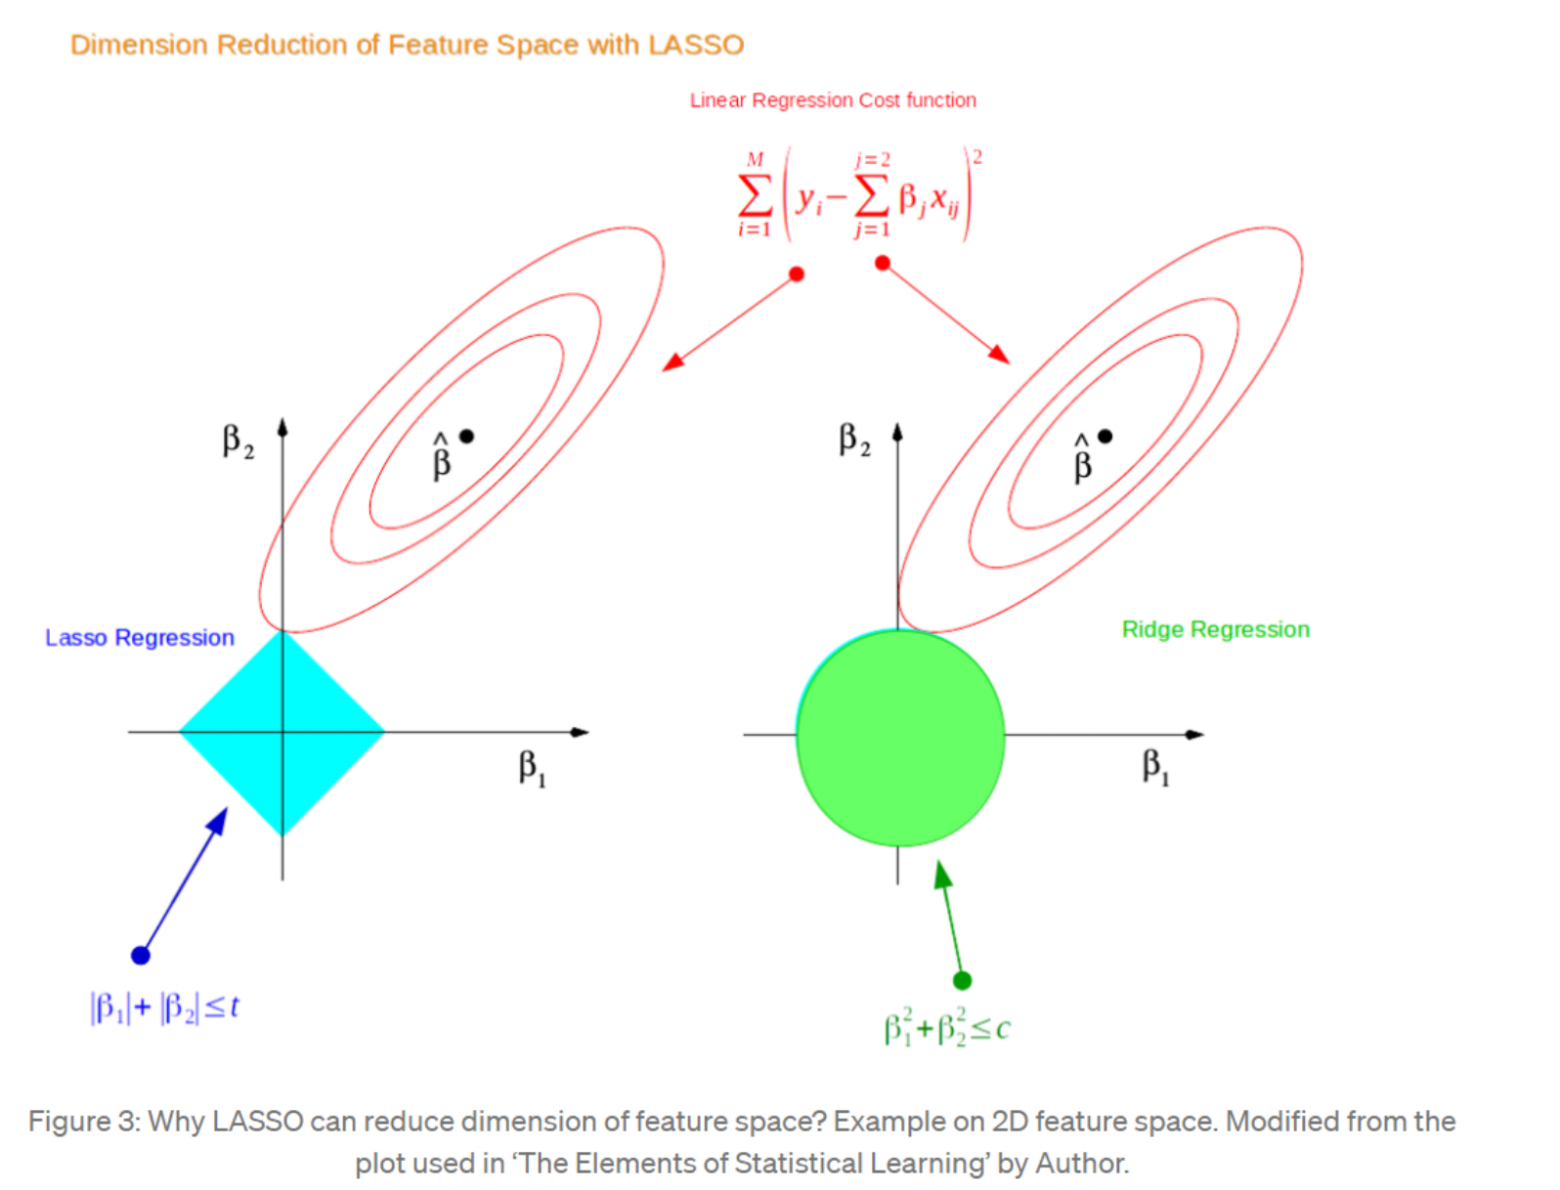
\includegraphics[width=1.1\textwidth]{../img/1}
				\end{figure}
			\end{column}
		\end{columns}
		\note{
			
		}
	\end{frame}
	
		\begin{frame}
		\frametitle{Преобразование признаков. АГК}	
		\begin{columns}
			\begin{column}{0.47\textwidth}
				
					В методе главных компонент строится минимальное число новых признаков, по которым исходные признаки восстанавливаются линейным преобразованием с минимальными погрешностями.
				
				
				
			\end{column}
			\begin{column}{0.5\textwidth}
				\begin{figure}[]
					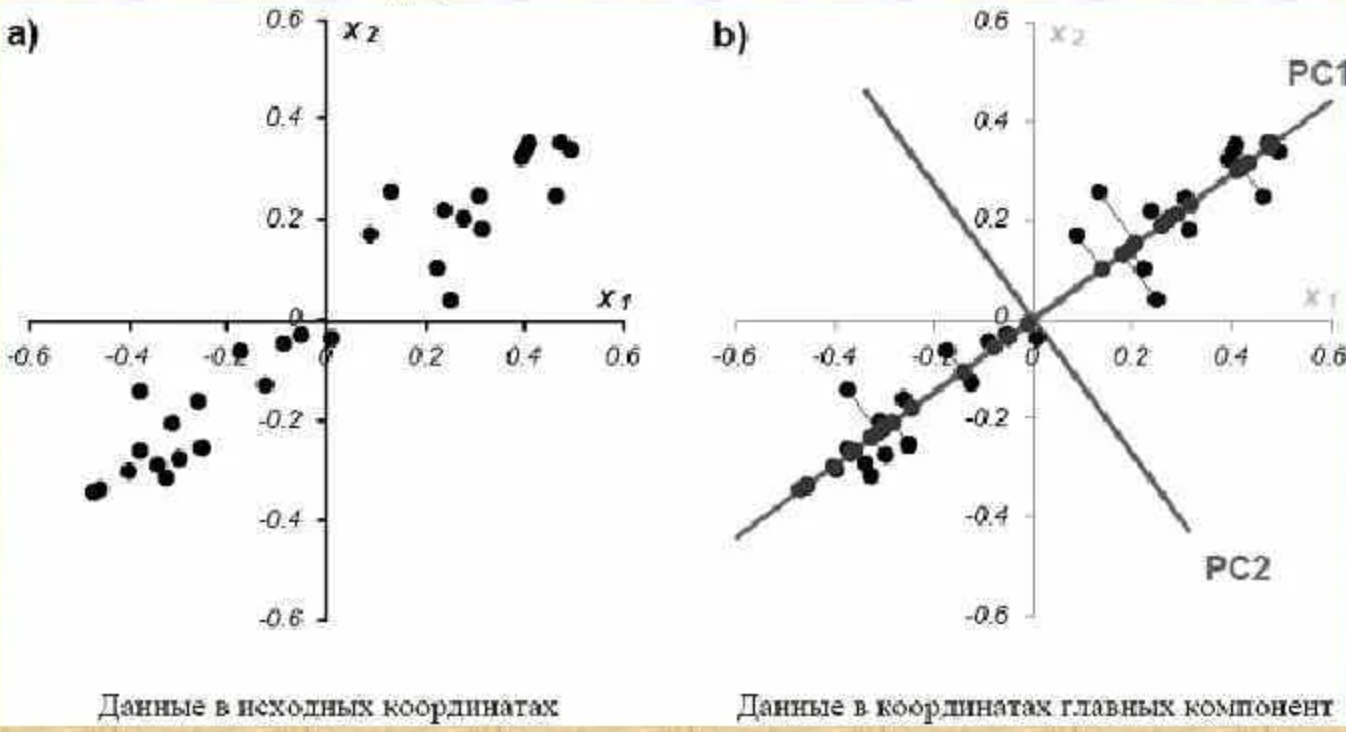
\includegraphics[width=1.1\textwidth]{../img/3}
				\end{figure}
			\end{column}
		\end{columns}
		\note{
			
		}
	\end{frame}
	
	\begin{frame}
		
	    \frametitle{Отбор признаков. Общий подход к выбору модели}
	
	Предположим, что есть некоторое семейство построенных моделей $\{\mathcal M_i\}_{i \in I}$.
	
	Хотим выбрать лучшую модель $\mathcal M^*$ для предсказания.
	
	\begin{center}
		\textbf{Классические методы выбора модели}
	\end{center} 
	
	\begin{itemize}
		\item Кросс-валидация
		\item Информационные критерии
		\begin{itemize}
		\item $\mathrm{AIC}_i = 2p_i - 2\ln{\mathcal L(\X; \mathcal M_i)}$
		\item $\mathrm{BIC}_i = p_i\ln{n} - 2\ln{\mathcal L(\X; \mathcal M_i)}$
		\end{itemize}
	
	\end{itemize}
	
	\end{frame}
	
	
	\end{document}
